\section{Some Example Tasks}
\label{sect:example_tasks}

We have designed some tasks to demonstrate the range of possibilities and showcase some of PAGI World's more unique features. Several of these tasks will be described next.

\subsection{The Piaget-MacGyver Room}
\label{sect:macgyver}

A prime example of a typical MacGyver task comes from Season 2, Episode 5 of the MacGyver television series. MacGyver found himself in a position where a mountain lion was threatening a friend of his. MacGyver, positioned at a ledge above his friend and the mountain lion, reconfigured some rocks and a log so that he could guide a nearby stream of water in such a way that it created a small waterfall separating his friend and the mountain lion. The mountain lion ran away immediately.

Of course, other solutions may have been available. Perhaps MacGyver could have simply thrown rocks at the mountain lion, or fashioned a bow and arrow out of twigs, sharpened stones, and parts of his knapsack. But these different solutions would have come with their own unique advantages and disadvantages, and furthermore, let us not lose sight of the PAGI-related question: Could an artificially intelligent agent figure out any of these solutions without having been specifically trained for that particular solution? PAGI problems such as the Piaget-MacGyver room challenge researchers to find answers to this question.

We can model this task in PAGI World as in Figure \ref{} %%%%%%ADD DESCRIPTION OF TASK AND IMAGE HERE

\subsection{Two Piagetian Tasks}

Some tasks which might be considered Piaget-MacGyver Rooms can come directly from classical Piagetian experiments. Inhelder and Piaget's (1958) Balance Beam Task (BBT) \cite{Inhelder1958} has been modeled many times using a variety of modeling techniques \cite{Wilkening1982,Sage1983,Shultz1994,Schmidt1996,Turner2002,Licato2012}. In the BBT, a balancing beam with a set of weights are provided to a subject. The balancing beam has notches, hooks, or some other apparatus that allows the weights to be placed on the left or right sides of the balancing beam at predefined intervals. In most versions of the task, the values of the weights and the distances that the locations are from the center are made available to the subject. The task is normally to figure out some version of the torque rule, which relates the product of the value of a weight and its distance from the center. For example, the subject may be presented with a configuration of weights on the scale, and the subject is asked to predict whether the right or left side will tilt downwards or the scale will balance.

We recreate the BBT in PAGI World as in Figure \ref{} %%%%%%%%%DESCRIBE implemented task

In the magnet test, also from \cite{Inhelder1958}, the subject is provided with a circular board with a rotating bar or needle in the middle. Surrounding the rotating bar are boxes which appear exactly the same except for a simple shape pictured on top of each box: either a circle, diamond, star, or square. Rotating the needle reveals that more often than not, it stops so that it is pointing to the star boxes. The subject is asked to explain why this is the case (it's because there is a magnet hidden inside of the star boxes), and is encouraged to experiment by for example moving the boxes around. Some explanations provided by subjects seem to display a form of Analogico-Deductive Reasoning (ADR) \cite{Bringsjord2012}.

The magnet test can be implemented in PAGI World by %%%%%%describe implemented task

One clear limitation of computationally modeling these Piagetian tasks is that you can't really communicate with the AI agent in natural language like you can with the children in Piagetian experiments. Although the current state of the art in natural language processing and generation prohibits such communication at present, PAGI World offers tools to make it easier for researchers who are trying to achieve this benchmark. There is a way to ``talk to" the AI agent through an input text box in PAGI World itself. Having the agent talk back, however, can be handled in two ways: through simple output handled completely by the code on the AI side, or by sending a message to PAGI World that can be displayed in an output window.

However, because it is difficult to give an AI agent complex instructions on how to perform a task (assuming that knowledge of what conditions constitute successful completion of a task aren't built in to the agent's code), PAGI World also allows for objects in the simulation to have an objective utility value. These are called \textit{endorphins}; objects with a positive endorphin value are those that the AI agent may want to pursue (e.g. food items), whereas negative endorphin values are those the agent should avoid. Most objects in PAGI World have an endorphin value of zero, and PAGI World itself does not ensure that certain endorphin-seeking behaviors are implemented by the agent. 

%\subsection{PERI psychometric tasks?}

%\subsection{Crow Intelligence Tasks}
%Wire Bending and Pebble Dropping
%Cockatoos can do it too http://news.sciencemag.org/plants-animals/2014/09/cockatoos-can-learn-each-other-how-make-and-use-tools
%- use Logic-based approach for this

In order to demonstrate the variety of AI approaches that can be used with PAGI World tasks, we will next describe some tasks for which we have also developed simple AI systems to solve those tasks. 

\subsection{Dancing Experiment}
Using the PAGI World environment, we set out to create an artificial intelligence agent that is capable of learning through reinforcement provided by a human teacher.  PAGI World allows the user to send commands to the agent via a small input box.  We used this feature to teach the agent how to perform a specific dance routine in an extremely brief training period.

The agent entered the world with little prior knowledge.  In fact, throughout the learning period, the amount of information known by the agent remained relatively constant.  The agent initially knew how to perform several dance moves, e.g.: a slide from one side to another, a jump with a 360-degree spin, and a dance move commonly referred to as `raising the roof.'  Additionally, the agent had a two-dimensional table of dance moves.  This move table, described in detail below, is intended to represent the agent's knowledge of how to combine the moves it knows, in order to perform dance routines.  The agent starts out with no real understanding of how to perform a cohesive dance, but through interaction with the user, the agent can learn any routine.


%INSERT MOVES
\begin{figure}[h]
	\centering
	\begin{subfigure}{.5\textwidth}
		\centering
		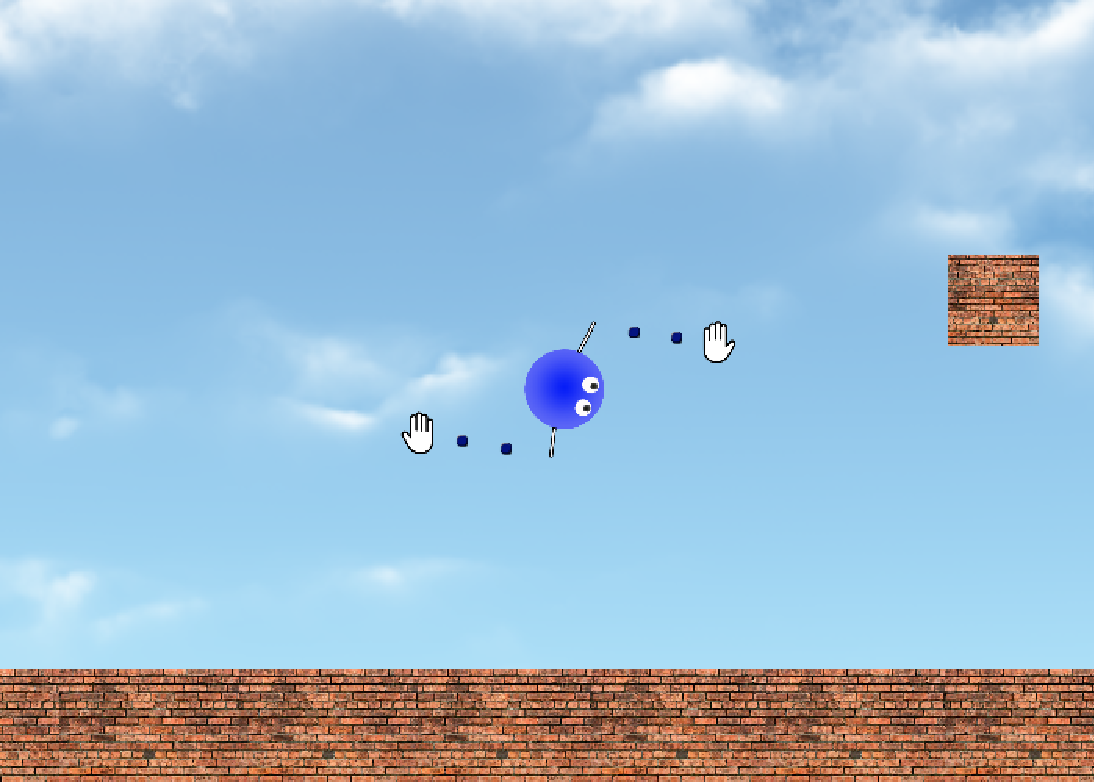
\includegraphics[width=.8\linewidth]{360cropped}
		\caption{Agent performing a Jump 360}
		\label{fig:sub1}
	\end{subfigure}%
	\begin{subfigure}{.5\textwidth}
		\centering
		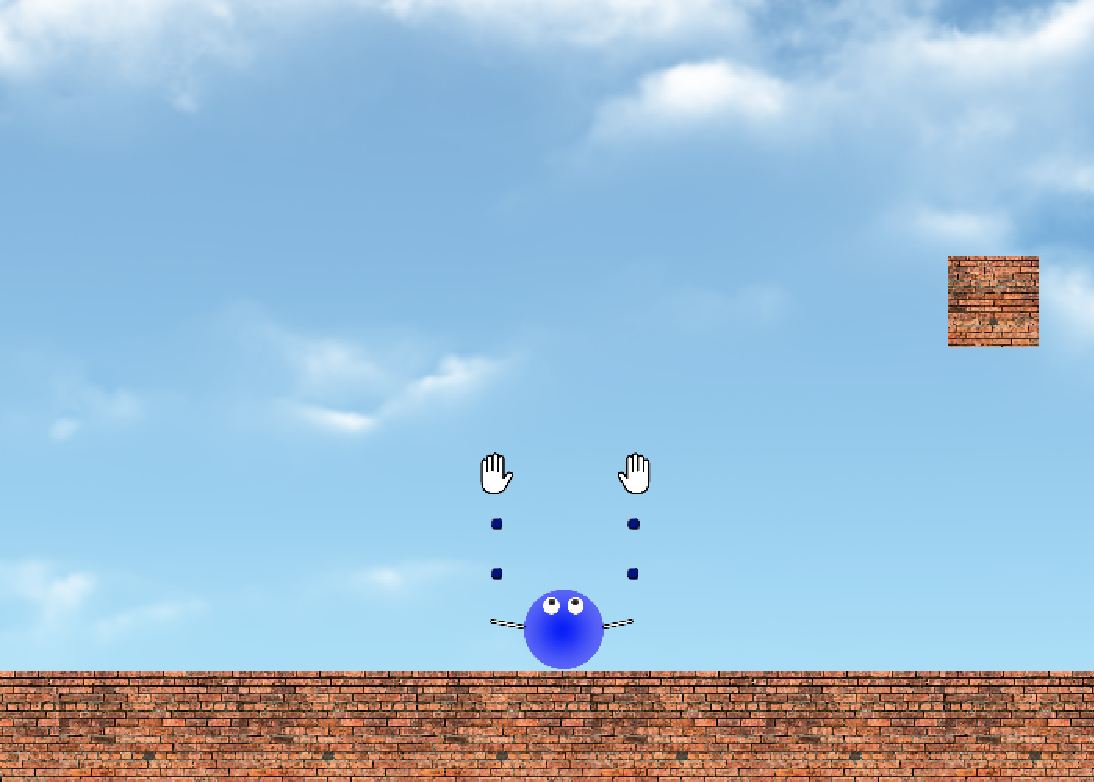
\includegraphics[width=.8\linewidth]{roofcropped}
		\caption{Agent 'raising the roof'}
		\label{fig:sub2}
	\end{subfigure}
	\caption {Agents performing pre-known dance moves}
	\label{fig:dances}
\end{figure}


Table \ref{unlearn} refers to an initial move table.  The top row denotes the current state of the agent, determined by which move the agent performed previously.  The `begin' column indicates the probability that a particular move being the first move of the sequence.  As you can see, the initial probability for any move to be selected as the first dance move is 0.25.  If, for example, move 3 was chosen to be the first move, the agent would then look under the move 3 column to select the next move.  Again, all these probabilities are equal, so the next move will be chosen at random.  The move selection process would continue in this fashion, until the dance to be performed is the correct length.

%INSERT TABLE 1 HERE
\begin{table}[h]
	\begin{center}
		\begin{tabular}{| c | c | c | c | c | c |}
		
		\hline
			 & begin & move 1 & move 2 & move 3 & move 4 \\	\hline	
			move 1 & 0.25 & 0.25 & 0.25 & 0.25 & 0.25 \\	\hline
			move 2 & 0.25 & 0.25 & 0.25 & 0.25 & 0.25 \\	\hline
			move 3 & 0.25 & 0.25 & 0.25 & 0.25 & 0.25 \\	\hline
			move 4 & 0.25 & 0.25 & 0.25 & 0.25 & 0.25 \\	 \hline
		
		\end{tabular} %
	\end{center}
	\caption {Example unlearned move table}
	\label{unlearn}
\end{table}
In order to get the agent to learn a dance, we used a first-order Markov chain.  This allowed the agent to remain essentially memory-less, as `first-order'�� implies that the agent'��s next action is based solely on its current state,�� or in our case, the move that came immediately before.  This could easily be extended to a higher order for more complicated dances or for other desired goals.

If you asked the agent to perform a 4-move dance initially, moves would be selected at random, as each move has an equal probability to be chosen regardless of what state the agent is in.  In order to begin teaching the agent, the user must tell the agent to enter learning mode. Learning mode begins with the agent generating all possible moves for all possible states, using iterative deepening depth first search.  The first moves in this sequence would be single moves; these are used to 'teach' the first move in the desired dance.  After these single moves, the agent would move on to two-move combinations.  The agent would perform a move from the tree, then await feedback from the user.  The user would respond with either `good' or `bad' using the text box built in to PAGI World.  The agent would store this feedback, and then continue on to the next move in the tree.  After the agent received feedback from all possible single moves/move combinations, the agent would begin to generate the new move table.  Each move for a particular state would receive a probability of $1/N$, where $N$ is the number of moves in that state that received positive feedback.  This table would then replace the move table previously in the agent's knowledge.

Table \ref{tab:learn1} demonstrates what the move table could look like after learning has occurred.  As before, the top row indicates the current state of the agent, and the probabilities a move will be chosen for a particular state corresponds to the row labeled accordingly.  In this table, move 2 is the only move that has a chance to be picked as the first move.  From there, the agent will move on to the `move 2' state to select the next move.  In this state, the only move that can be chosen is move 3.  The agent will continue selecting moves in this fashion, until the dance is of the correct length, in this case, a 4 move dance.

%INSERT TABLE 2 HERE
\begin{table}[h]
	\begin{center}
		\begin{tabular}{| c | c | c | c | c | c |}
		
			\hline
			 & begin & move 1 & move 2 & move 3 & move 4 \\	\hline	
			move 1 & 0 & 0 & 0 & 0 & 0 \\	\hline
			move 2 & 1 & 0 & 0 & 0 & 1 \\	\hline
			move 3 & 0 & 1 & 1 & 0 & 0 \\	\hline
			move 4 & 0 & 0 & 0 & 1 & 0 \\	 \hline
		\end{tabular} %
	\end{center}
	\caption {Example learned move table}
	\label{tab:learn1}
\end{table}
Noise can be interjected into the agents move table simply by giving multiple moves within a single state positive feedback.  This would allow $N$ moves to be selected at a single state, provided these $N$ moves were all given `good' as feedback during the learning process.  This would give the agent a little more freedom in the dance that selected.  Feedback given in this manner could allow the agent to perform a `freestyle' dance, while allowing only one move to be selected at a particular state (as in table \ref{tab:learn1}) would call for a specific routine.  Below is an example of a `freestyle' move table.

\begin{table}[h]
	\begin{center}
		\begin{tabular}{| c | c | c | c | c | c |}
			\hline
			 & begin & move 1 & move 2 & move 3 & move 4 \\	\hline	
			move 1 & 0.33 & 0.5 & 0 & 0 & 0.25 \\	\hline
			move 2 & 0.33 & 0 & 0.33 & 0 & 0.25 \\	\hline
			move 3 & 0 & 0.5 & 0.33 & 0 & 0.25 \\	\hline
			move 4 & 0.33 & 0 & 0.33 & 1 & 0.25 \\	 \hline
		
		\end{tabular}  %
	\end{center} 
	\caption{Example learned move table with noise}
	\label{tab:learn2}
\end{table}

Using the tools outlined above, we were able to successfully teach the agent how to dance.  The agent started out with zero knowledge on how to combine his dance moves into a cohesive dance, and after learning the agent could successfully dance any time he was asked.  This simple example demonstrates the simplicity of interacting with an AI agent through verbal�� commands in PAGI World. 
%another task believed to demonstrate animal intelligence...talk about dogs

\subsection{Operant Conditioning Chamber and Classical Conditioning}

There are multiple kinds of learning a successful AGI system can make use of; this environment focuses on Classical Conditioning using a na\"{i}ve Bayesian probability model.

An Operant conditioning chamber (also called a Skinner box) is an apparatus used in the study of animal behavior. %Jack, although these concepts are well-known in psychology, we still need to cite something here. Can you figure out what we need to cite?
Operant conditioning chambers contain at least one operandum (typically a lever) and a means of delivering a primary reinforcer (a reward/punishment pair, e.g. apple/poison). Some operant chambers incorporate lights, sounds and/or drawings to produce multiple stimuli and signify when food is available.

It is easy to construct an operant conditioning chamber in PAGI World. A dispenser is placed within grabbing distance of the agent which when grabbed can produce a primary reinforcer (apples or poison).  These objects have associated positive and negative `endorphins' which the agent can respond to just as an animal would. 


\begin{figure}[h]
\centering
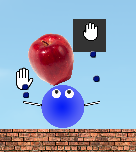
\includegraphics{dispenser}
\caption{PAGI World Operant Conditioning Chamber.} %expand on this caption a little---describe what we're looking at. Same applies to the next figure's caption.
\end{figure}


The application of such an environment is to test classical conditioning algorithms before full scale deployment.  One can limit the number of variables and focus solely on the agent's ability to interpret conditioned stimulus (CS)/unconditioned stimulus (US) pairs.

One such classical conditioning algorithm is implemented using a na\"{i}ve Bayesian probability model. %same here: please find out what a good citation is for this. Wikipedia itself isn't a good source, but it might point you to academic papers that are.
 The agent starts with the assumption that no action of his will lead to endorphins.  Once placed in the operant conditioning chamber, the agent tries to interact with the dispenser.  If this interaction with the dispenser produces endorphins, the CS-US pair is strengthened.  The strength of this CS-US pair is measured as a probability.

The agent is run through a number of tests, each time able to grab the dispenser a set number of times, or for a set period of time.  At the end of each trial, probabilities and the history of the dispenser are saved in a memory file to be used as the initial cases for the next trial.  PAGI World also has built in functions that allow one to change the dispenser's qualities.  This is used to replicate the phenomenon of extinction. %citation for extinction required. An introductory psychology textbook might suffice.


\begin{figure}[h]
\centering
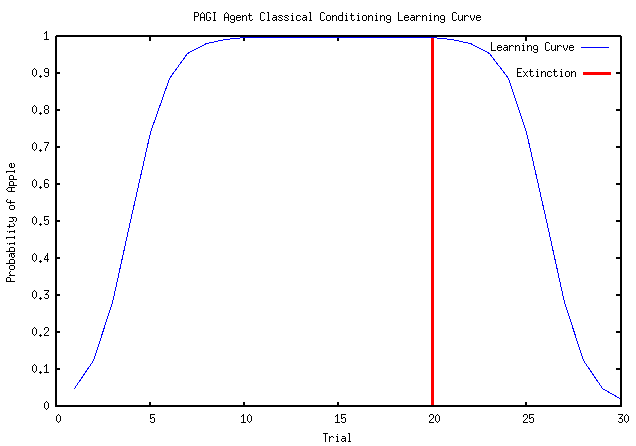
\includegraphics[scale=0.5]{cc_graph}
\caption{Agent Learning Curve}
\end{figure}

In this experiment the agent was provided with a dispenser that produced apples on every grab.  The graph shows the agent coming to this conclusion, as the probability of the dispenser dropping an apple rises to nearly one.  However, after 20 trials the dispenser is turned off.  The conditioned stimulus (grabbing the dispenser) is no longer paired with the conditioned response (endorphin increase due to apple).  Thus, a gradual weakening of the conditioned response can be observed, expressed on the graph as the decrease in the probability of an apple falling.  

This is just one simple example of the flexibility of PAGI World.  Both the operant conditioning chamber and example classical conditioning algorithm could be expanded to be more functional. %in what ways?